\subsection{Software Engineering}\label{chap:softwareEngineering}
What is software engineering?  How does software engineering related to the
student learning objectives of being able to ``use the steps of the software
development process to create high-quality software''.  Summarize the key
topics.

Give an overview of this section.  What work samples will you include?
(You must include at least two.)  You can cite any references like
this~\cite{parks:samsfsoal:2009}.

\subsubsection{Name of Work Sample 1}
Give an introduction for the work sample and explain its context.  The
introduction for the work sample must be at least 50 words.

The work samples must address the student learning objectives addressed in
this section.  A work sample may be used to address more than one student
learning objective.  If you use the same work sample to address multiple
objectives, put it in the Appendix and reference it here.
There are a range of possible work that might be
included as work samples including parts of the software develop process
for a particular program (e.g., requirements specification, design documents,
test suites, and the program code itself), papers written, and
experimental or theoretical studies.  The work samples need not only
be from the current course.  You should remember to save your work when
you finish a course so that you can use that work as a work sample in
your portfolio later.

Depending on the length of the work sample, you may include it in-line in
this section, or include it in the appendix.  Listing~\ref{lst:sampleWorkSample4}
is an example of how to include a work sample in-line. (And that's how you
link to it.)

\begin{singlespace}
\begin{lstlisting}[float,
                   escapeinside='',
                   basicstyle=\ttfamily\footnotesize,
                   emphstyle=\textbf,
                   numberstyle=\tiny,
                   xleftmargin=.3cm,
                   language=java,
                   numbers=left,
                   numbersep=5pt,
                   firstnumber=auto,
                   stepnumber=1,
                   numberblanklines=true,
                   showspaces=false,
                   showstringspaces=false,
                   showtabs=false,
                   captionpos=b,
                   caption=Sample Java Source File,
                   label=lst:sampleWorkSample4]
public class Hello {
    public static void main(String[] args) {
        System.out.println("Hello, World!");
    }
}
\end{lstlisting}
\end{singlespace}

Here, some of your work samples might be diagrams.  For example,
Figure~\ref{fig:doctorUseCase3} is a use case diagram for a patient tracking
system. (And that's how you link to it.)

\begin{figure}
    \centering
    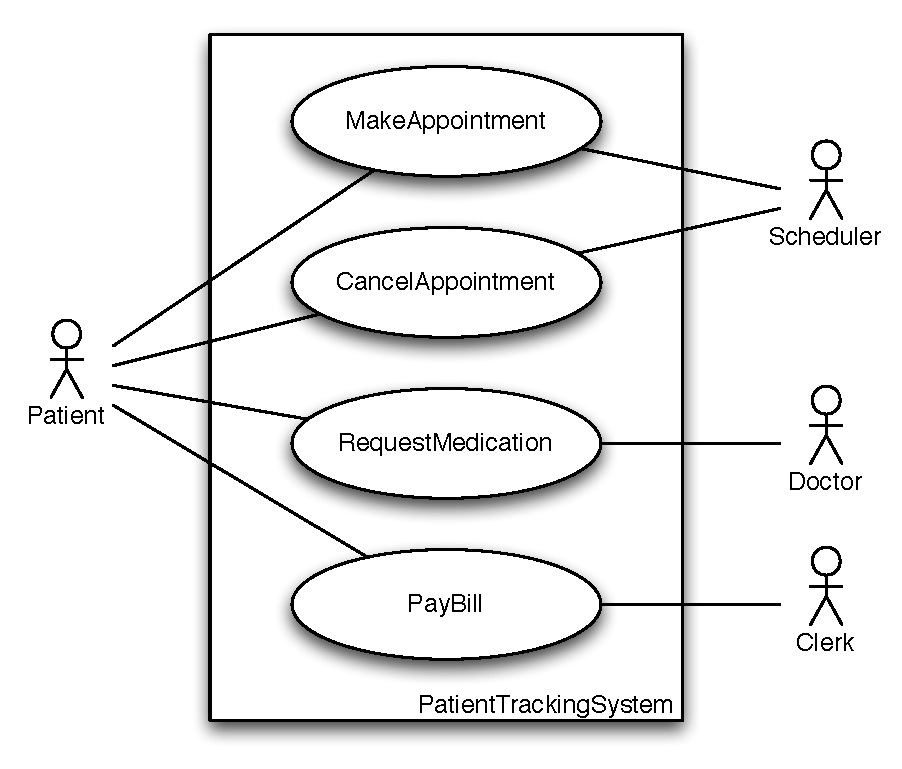
\includegraphics[width=4in]{figures/DoctorsOfficeUseCase}
    \caption{PatientTrackingSystem Use Case}
    \label{fig:doctorUseCase3}
\end{figure}

\subsubsection{Name of Work Sample 2}
Give an introduction for the work sample and explain its context.  The
introduction for the work sample must be at least 50 words.

Appendix~\ref{chap:appendixA} includes a long work sample.  (And that's how you
link to it.)

\subsubsection{Reflection}
In this section, you are to explain in your own words:
\begin{enumerate}
\item Your view of the meaning of the student learning objective
\item What aspect of each work sample addresses this student learning
      objective
\item An honest and accurate appraisal of your strengths and weaknesses at
      this point in your career with respect to this SLO.  It is unlikely
      that you have no weaknesses and it is also unlikely that you have no
      strengths with respect to this SLO.
\end{enumerate}

The length of this subsection must be at least 500 words.
